\documentclass[12pt]{article}
\usepackage{graphicx}
\usepackage{subcaption}
\usepackage[]{mcode}
\usepackage{mwe}
\usepackage{amsmath}
\usepackage[T1]{fontenc}


\DeclareMathOperator{\erf}{erf}
\renewcommand{\thesubsection}{\thesection.\alph{subsection}}

\begin{document}

\title{CMSC 460 - HW7}
\author{Gudjon Einar Magnusson}

\maketitle

%6.1
\section{}

\begin{center}
 \begin{tabular}{l c c c c c} 
 $f(x)$ & $a$ & $b$ & $tol$ & Itter & Value \\
 \hline

 $humps(x)$ & 0 & 1 & $10^{-4}$ & 93 & 29.8583 \\ 
 $humps(x)$ & 0 & 1 & $10^{-6}$ & 265 & 29.8583 \\
 $humps(x)$ & -1 & 2 & $10^{-6}$ & 165 & 26.3450 \\
 $\sin(x)$ & 0 & $\pi$ & $10^{-8}$ & 121 & 2.0 \\
 $\cos(x)$ & 0 & $(9/2)\pi$ & $10^{-6}$ & 241 & 1.0 \\
 $\sqrt{x}$ & 0 & 1 & $10^{-8}$ & 153 & 0.6667 \\
 $\sqrt{x} \log x$ & eps & 1 & $10^{-8}$ & 205 & -0.4444 \\

 $\tan(\sin x) - \sin(\tan x)$ & 0 & $\pi$ & $10^{-8}$ & ? & ? \\
 $\tan(\sin x) - \sin(\tan x)$ & 0 & $\pi$ & $10^{-4}$ & 505 & 2.6644 \\

 $1/(3x-1)$ & 0 & 1 & $10^{-4}$ & ? & ? \\ 

 $x^{8/3}(1-x)^{10/3}$ & 0 & 1 & $10^{-8}$ & 73 & 0.0074 \\ 
 $x^{25}(1-x)^2$ & 0 & 1 & $10^{-8}$ & 49 & 0.0001 \\ 

\end{tabular}
\end{center}

In general the evaluation points are concentrated at peaks and valleys of the function.

$f(x) = \tan(\sin x) - \sin(\tan x)$, $x \in [0, \pi]$ fails to converge in a reasonable time because function fluctuates wildly close to $x=\frac{\pi}{2}$ where $\tan x$ shoots to infinity.

$f(x) = 1/(3x-1)$, $x \in [0, 1]$ gets stuck and fails at $x=\frac{1}{3}$. On either side of that point $f(x)$ shoots to infinity and negative infinity. Evidentially it fails with a division by zero.


%6.2
\section{}
%fuuu

%6.3
\section{}

The error drops quickly as $n$ increases. Figure \ref{fig_pi_err} shows the error as a function of $n$.

\begin{figure}
    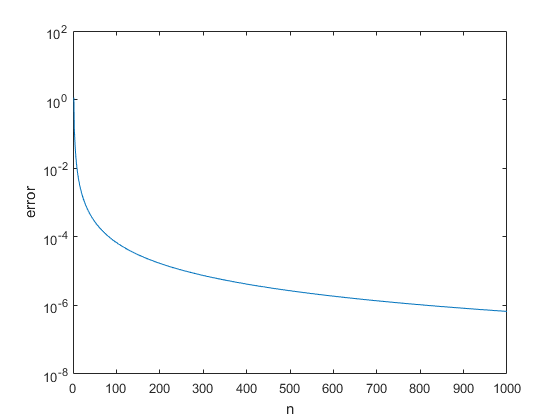
\includegraphics[width=\linewidth]{pi_err2}
    \centering
    \caption{Error of approximating $\pi$ using the composite trapezoid rule with $n$ equally spaced points}
    \label{fig_pi_err}
\end{figure}


\end{document}